\documentclass[oneside, a4paper, onecolumn, 11pt]{article}

% Change this: Customize the title, author, advisor, abstract
\newcommand{\thesistitle}[0]{Falling Sand Simulation}
\newcommand{\authorname}[0]{Alisa Karlova, Eugenio Animali, Victor Martin}

\usepackage[
  left=2cm,top=2.0cm,bottom=2.0cm,right=2cm,
  headheight=17pt, % as per the warning by fancyhdr
  includehead,includefoot,
  heightrounded, % to avoid spurious underfull messages
]{geometry}


\usepackage[T1]{fontenc}
\usepackage{float}
\usepackage{amstext}
\usepackage{amsmath}
\usepackage{amssymb}
\usepackage{url}
\usepackage{graphicx}
\usepackage{wrapfig}
\usepackage{enumerate}
\usepackage{paralist}
\usepackage{xspace}
\usepackage{color}
\usepackage{times}
\usepackage{booktabs}
\usepackage[colorlinks,linkcolor=blue]{hyperref}
\usepackage[colorinlistoftodos,prependcaption,textsize=normal]{todonotes}
\usepackage{pdfpages}
\usepackage{fancyhdr} %% For changing headers and footers

\usepackage{titling}
\usepackage[nottoc,numbib]{tocbibind}

%% \predate{}
%% \postdate{}
%% \date{}
%% \author{\authorname}


\begin{document}

%\title{\thesistitle}

%\maketitle

% Max 10 lines.
%\noindent \paragraph*{Abstract}
%\abstract

\begin{center}

\includegraphics[width=0.65\textwidth]{logo-EP-vertical}

\vspace*{2em}
%
{\large
\textbf{\'Ecole Polytechnique}

\vspace*{1em}
\textit{Concurrent and Distributed Computing Final Project}


\vspace*{3em}
{\Huge \textbf{\thesistitle}}
\vspace*{3em}



\textit{Authors:}

\vspace*{1em}
\authorname{}}

\end{center}

\vfill
\hspace{0pt}

\newpage



% Setting up the header
\pagestyle{fancy}
%\renewcommand{\headrulewidth}{0pt} % Remove line at top
%\renewcommand{\headrulewidth}{0.4pt}% Default \headrulewidth is 0.4pt
\lhead{\authorname}
%\chead{\acronym}
\rhead{\thesistitle}



\newpage
\tableofcontents
\newpage

%\pagenumbering{arabic}

\section{Introduction}

In this report we log and describe the progress of the Falling Sand Simulation Project undertaken by the authors during the third year as Bachelors in Computer Science and Mathematics at Polytechnique, France.

\section{Initial Ideas and Design}

By playing around with falling sand simulations, which happen to be plentiful online, one can get an initial idea of the fundamental algorithm that defines the animation of this simple project. Let us define our initial intentions.

\subsection{Visual elements}

Our first version will look as follows: The Scene is a grid of black and white square cells, where white cells indicate the presence of sand particles in a black vacuum. Let the sand particle in the current frame be in cell 5 in Figure~\ref{fig:adjacent}. When there is no obstruction (more sand or Scene edge) in cell 8, it will fall down by one cell per frame.

\begin{figure}
    \centering
    \includegraphics[width=0.5\linewidth]{adjacent_grid.png}
    \caption{Adjacent cells}
    \label{fig:adjacent}
\end{figure}

To create an effect similar to that one sees in sand dunes, we implement the following physics. If cell 8 is occupied, we choose order to check the cells 7 and 9, and for the first of these that is free, our sand particle moves there for the next frame. This avoids tall towers of sand with a wall edge, which doesn't happen in real sand, instead degenerating to a pyramid shape. Indeed, if all 7, 8 and 9 are occupied, this algorithm keeps the sand particle fixed, making sand dune shapes stable. Lastly, when a cell does not have an adjacent cell due to reaching a border of the Scene, this is considered as an occupied cell.

This is a naive first design with several flaws. Firstly, it allow for loss of mass. Say in one frame there is a particle in cells 4, 5 and 8, and that below 8 is the border of the Scene. Then in the following frame, the particle in 4 will fall to 7, but 5 may also fall to 7, as 8 is occupied. This suggests we need either communication between threads during 


\section{Sequential CPU Implementation}

\subsection{Grid Representation}

The simulation state is a fixed-size, dense grid of cells, each storing one of three values:
\begin{itemize}
    \item \texttt{Empty}
    \item \texttt{Sand}
    \item \texttt{Wood}
\end{itemize}
as a \texttt{std::uint8\_t} enum (\texttt{CellType}).
The grid is backed by a single row-major

\texttt{std::vector<CellType>} of length $\mathit{width} \times \mathit{height}$, with cell $(r,c)$ stored at index $r \cdot \mathit{width} + c$.
Row~0 is the top of the grid; sand falls in the direction of increasing row index.

Two access paths are provided.
\begin{enumerate}
    \item The unchecked \texttt{cell(row,\,col)} returns a direct reference into the backing vector and is used in the hot update loop, where the caller guarantees valid bounds.
    \item The bounds-checked \texttt{at(row,\,col)} is used elsewhere and encodes a deliberate convention: any out-of-bounds read returns \texttt{Wood}.
\end{enumerate}

Because \texttt{Wood} is the immovable cell type, this makes all four edges of the grid behave as solid walls without special-casing in the update rule---a grain that queries the cell ``below'' the bottom row sees \texttt{Wood} and therefore does not move.
The matching \texttt{set(row,\,col,\,t)} silently ignores out-of-bounds writes.
Together, these two conventions guarantee that no sand can leave the domain, which is the basis of the conservation property we verify later.

Scene initialisation uses \texttt{seed\_blob(row,\,col,\,radius,\,t)}, which stamps a filled disk of a given cell type via a squared-distance test ($\delta r^2 + \delta c^2 \leq r^2$), avoiding a square root.
Conservation checks use \texttt{count(t)}, a linear \texttt{std::count} over the buffer.

\subsection{The Update Rule and the Snapshot Mechanism}

A single simulation step is implemented in \texttt{Simulation::step(Grid\&)}.
The movement rule applied to a sand grain at $(r,c)$ follows a fixed priority order:

\begin{description}
    \item[Straight down.] Move to $(r{+}1,\,c)$ if that cell is empty.
    \item[Both diagonals free.] Choose one of $(r{+}1,\,c{-}1)$ or $(r{+}1,\,c{+}1)$ uniformly at random.
    \item[One diagonal free.] Move into whichever of the two diagonal cells is empty.
    \item[Blocked.] The grain stays in place.
\end{description}

Sand moves only into the row directly below it, so each step advances any falling grain by at most one row.

Crucially, the step does not read and write the same grid.
At the start of each step a full copy of the backing buffer is taken (\texttt{current = g.data()}); all movement decisions are made by reading from this immutable snapshot through a local \texttt{read(r,\,c)} helper (which, consistent with \texttt{at}, returns \texttt{Wood} for out-of-bounds coordinates).
Writes, however, go directly into the live grid~\texttt{g}.
This is therefore \emph{not} a ping-pong double buffer in which two full grids are swapped each frame; it is a single live buffer mutated in place, paired with a read-only snapshot of the frame's initial state.
The snapshot costs one $O(\mathit{width} \times \mathit{height})$ allocation and copy per step; this overhead could be amortised by reusing a pre-allocated member buffer.

Because all grains read their neighbourhood from the same start-of-frame snapshot, the visit order cannot affect what any individual grain perceives.
What visit order \emph{can} affect is contention for destination cells, which is handled separately (Section~\ref{sec:conflict}).

The grid is scanned from row $\mathit{height}-2$ upward to row~$0$; the bottom row is omitted since grains there have nowhere to fall.
Scanning bottom-up ensures that by the time any row is processed, the row beneath it is already finalised for the current step. Combined with the downward-only movement rule, no grain can be written into a cell during the same step in which it is being read as a source.
An additional guard 

\[\texttt{if (g.cell(r,\,c) != Sand) continue} \]

tests the live grid inside the loop; under the current scheme this is redundant, but it is cheap and defensive.

\subsection{Conflict Resolution and Bias Control}
\label{sec:conflict}

Two distinct grains visible in the snapshot can independently select the same destination cell. For example, a grain at $(r,c{-}1)$ choosing down-right and a grain at $(r,c{+}1)$ choosing down-left, both targeting $(r{+}1,c)$.
This is resolved by \emph{first-writer-wins}: a grain commits its move only if the destination cell is still \texttt{Empty} in the live grid at the moment of writing (checked via a \texttt{next\_at} helper that reads~\texttt{g}, not the snapshot).
If an earlier grain in the scan has already claimed that cell, the later grain finds it occupied and stays in place.
This mechanism prevents two grains from collapsing into one cell and is therefore central to the conservation guarantee.

First-writer-wins alone introduces an order dependence: whichever grain is visited first wins contested cells, so a fixed left-to-right scan would systematically favour one side.
Two independent symmetrising mechanisms counteract this.

\paragraph{Per-grain randomisation.}
When a grain has both diagonals available and no straight-down option, the direction is chosen by a fair coin flip: \texttt{(rng\_() \& 1u) ? -1 : +1}, drawn from a \texttt{std::mt19937} Mersenne Twister owned by the \texttt{Simulation} object and seeded deterministically (default seed \texttt{0xC5E305}).
Owning the RNG makes runs fully reproducible given the seed.

\paragraph{Scan-direction alternation.}
The per-step flag \texttt{reverse\_cols = (steps\_ \& 1)} flips the column traversal order on every step: even steps scan left-to-right, odd steps right-to-left.
Any directional preference introduced by first-writer-wins on one step is thus mirrored on the next, so the two biases tend to cancel over consecutive steps.

The two mechanisms address distinct sources of asymmetry: the RNG handles the per-grain tie, while scan-parity alternation corrects the global traversal order.

\subsection{Cost Characteristics}

The work performed in a step is data-dependent.
The outer loop visits $\mathit{width} \times (\mathit{height}-1)$ cells, but the body short-circuits immediately on any non-sand cell, so empty space and static wood are skipped at the cost of a single comparison.
Neighbourhood reads and potential writes are triggered only by actual sand grains.
Consequently, the cost of a step scales with the number of active sand grains, not merely with the grid area: a sparse grid is cheap to advance, and cost grows proportionally with density.
The one fixed per-step overhead independent of density is the full-buffer snapshot copy described in Section~\ref{sec:snapshot}.

This density-sensitivity is precisely what experiment 1b) in Section~\ref{sec:exp1b} is designed to expose, and it contrasts directly with the GPU implementation, whose per-block work is fixed regardless of cell contents.

Finally, one step corresponds to at most one row of downward motion per grain.
This establishes the physical-time unit against which step counts and throughput are later interpreted, and it differs from the Margolus phase used on the GPU. This distinction matters when comparing wall-clock timings and when choosing step counts for settling experiments.


\section{GPU Implementation: Framework and Architecture}

\subsection{Parallel CA and complications}

On a GPU the natural unit of work is one thread per cell, all running simultaneously. But in this game a direct translation of the sequential rule breaks down because neighbouring cells share state.
Two threads writing to the same destination cell in the same parallel pass may either merge two grains into one or silently erase one: both outcomes violate the conservation invariant.

Two standard remedies exist:
\begin{enumerate}
    \item \textbf{Double buffering}: read from one full copy of the grid, write to a second, then swap. This eliminates read/write races but doubles memory usage and still requires an atomic or priority scheme to resolve two grains targeting the same destination.
    \item \textbf{Disjoint partitioning}: partition the grid so that no two concurrent threads can write to the same cell. With disjoint write sets, the update proceeds in place on a single buffer with no extra memory and no atomics. The Margolus neighbourhood provides exactly this partition, and is the approach used here.
\end{enumerate}

\subsection{The Margolus Neighbourhood}

The Margolus scheme tiles the grid into non-overlapping $2\times 2$ blocks and updates each block independently.
Because the blocks are disjoint, a transition rule that maps the four cells of a block only to those same four cells can be applied to all blocks simultaneously, as the write sets are disjoint by construction.

A single fixed tiling cannot move a grain across a block boundary, so the partition is shifted between passes: cycling the block origin through four offsets,
\[
  (0,0),\quad (-1,-1),\quad (0,-1),\quad (-1,0),
\]
ensures that every pair of adjacent cells eventually falls within a common block.
One full cycle through these offsets constitutes a logical simulation step; each individual dispatch (one offset) is a \emph{phase}.

The transition rule is a lookup table: the four cells of a block, each empty or occupied, define a small number of possible input configurations, each mapped to an output configuration chosen to mimic gravity.
Because the rule is a deterministic table lookup with no random component, a given initial grid and phase sequence always produce the same result.

\subsection{Mapping the Automaton onto the Compute-Shader Model}

The grid state lives in GPU memory as a single \texttt{RGBA32F} storage image, with the red channel encoding cell state ($1.0$ = sand, $0.0$ = empty).
For each phase, the host pushes the current offset and grid dimensions to the shader as a push constant, then dispatches a grid of $16\times16$ workgroups sized to cover all $\frac{W}{2} \times \frac{H}{2}$ blocks (one invocation per $2\times2$ block).
Consecutive phases are separated by a pipeline barrier that ensures all writes from one phase are visible before the next begins.

\subsection{Project Architecture}

The GPU implementation is a Godot~4 project (\texttt{godot\_project/}) structured so that the simulation shader, the interactive viewer, and the benchmarking harness are kept separate.

\begin{itemize}
    \item \textbf{\texttt{sand.glsl}} --- the compute shader containing the Margolus update rule.
    This is the single source of truth for the GPU simulation's behaviour: the lookup tables, per-block logic, and boundary handling all live here.
    Both the interactive viewer and the benchmark harness compile and dispatch this same shader, so the two cannot diverge in their physics.

    \item \textbf{\texttt{texture\_rect.gd}} --- the interactive front-end.
    It sets up the rendering device, compiles \texttt{sand.glsl}, seeds the initial scene, and advances the simulation in response to keyboard input (run/pause and single-step).
    The grid's storage image is bound directly as the displayed texture, so what appears on screen is the live simulation buffer.
    This path is used for visual inspection and debugging, not for measurement.

    \item \textbf{\texttt{benchmark.gd}} --- the headless measurement harness.
    It runs without a window, driving \texttt{sand.glsl} through a local \texttt{RenderingDevice} so that GPU work can be submitted and synchronised explicitly.
    It mirrors the structure of the C++ benchmark (Section~\ref{sec:cpu_bench}): identical scene seeding, untimed warm-up phases, then a single timed span over a fixed number of steps, followed by a conservation check.
    It also implements the symmetry-measurement mode used in Experiment~2, reporting left/right grain counts and their relative difference.
    Timing output is emitted as a single machine-readable key-value line parsed by the sweep scripts.
\end{itemize}


\section{Experiment 1 --- Throughput scaling}
\label{sec:exp1}

The throughput metric on both implementations is the nominal cell-updates
per second
\[
  \mathrm{CUPS} \;=\;
  \frac{\text{width}\times\text{height}\times\text{steps}}
       {\text{elapsed\_s}},
\]
defined identically irrespective of internal per-step work. A
``step'' is one CPU sweep (at most one row of fall per grain) or one
Margolus phase on the GPU. CUPS is therefore a measure of how fast the
grid is advanced one nominal step, not of useful work performed; for
this reason elapsed time is reported alongside CUPS, and speedup is
defined as the elapsed-time ratio $S = t_{\mathrm{CPU}}/t_{\mathrm{GPU}}$.

\subsection{Experiment 1a --- Grid-size scaling}
\label{sec:exp1a}

\paragraph{Setup.}
Square grids of size $N\in\{64,128,256,512,1024,2048,4096\}$ are run with
$\text{steps}=500$, $\text{warmup}=5$, and 10 repetitions per
configuration, on the standard three-blob sand scene (no wood). Per
configuration the median elapsed time and median CUPS are reported,
with the interquartile range as error band, to suppress the
right-skewed tail introduced by OS and driver scheduling. GPU timing
spans one explicit \texttt{submit}/\texttt{sync} around the whole
batch (\texttt{chunk=0}); each step is its own compute list, so the
storage-image barrier ordering consecutive Margolus phases is included
in the measurement. 

\paragraph{Results.}


\begin{center}
  \begin{tabular}{ccc}
  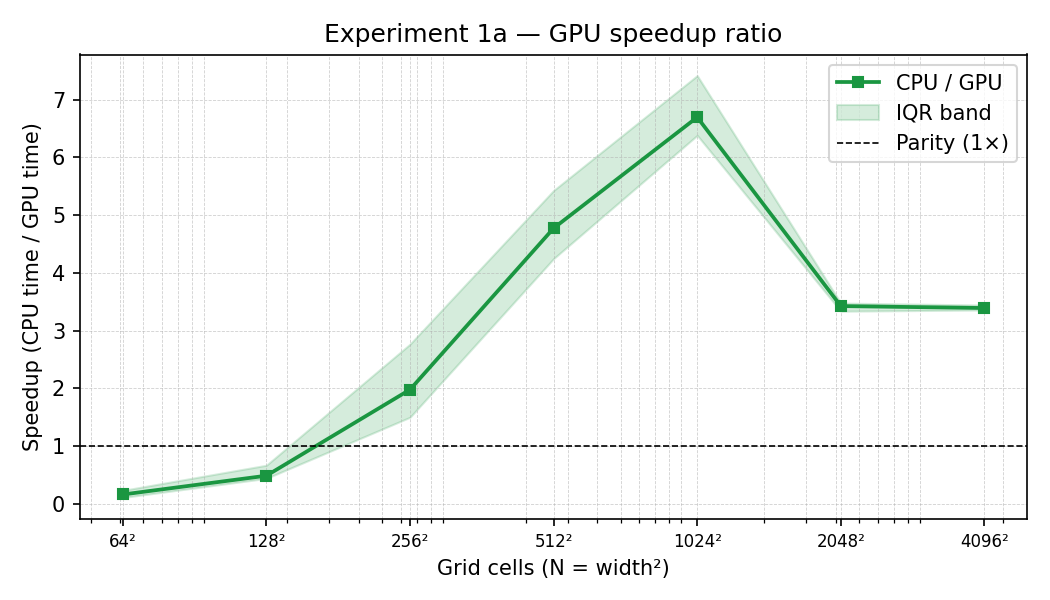
\includegraphics[width=0.4\linewidth]{figures/exp1a/exp1a_speedup.png} &
  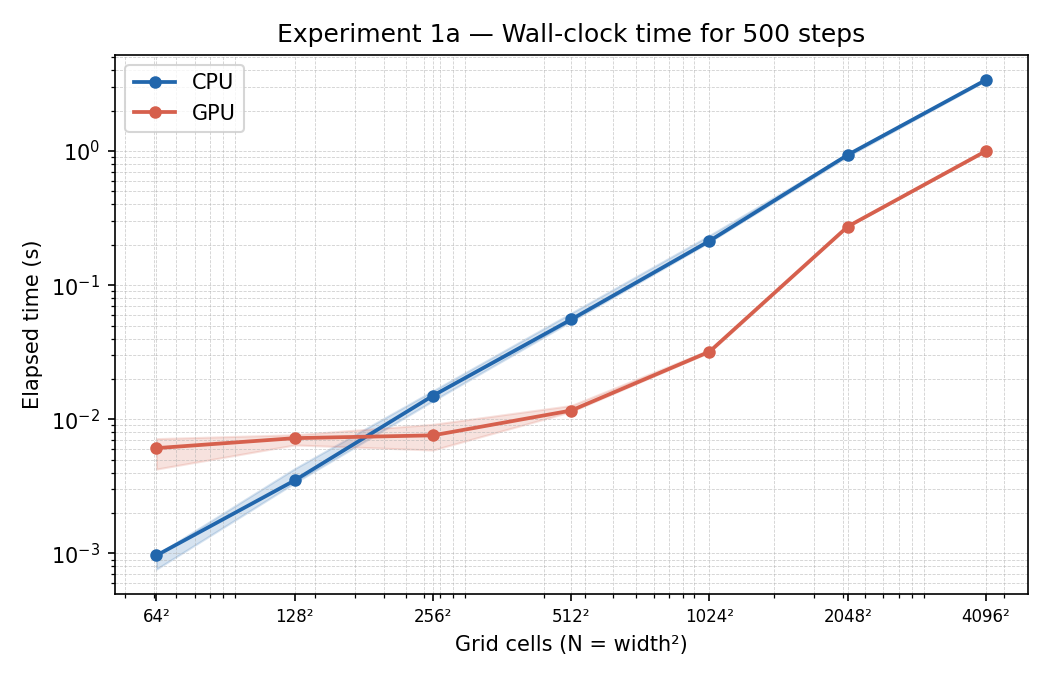
\includegraphics[width=0.4\linewidth]{figures/exp1a/exp1a_elapsed.png}
  \par\smallskip
  \label{fig:exp1a_speedup}
  \end{tabular}
\end{center}

The GPU only overtakes the CPU above roughly $200^2$ cells: at small grids it is overhead-bound (per-step dispatch and the image barrier dominate, and the SMs are not filled), so the CPU baseline is actually faster. Speedup peaks at $\sim\!6.7\times$ around $1024^2$ and then falls back to $\sim\!3.4\times$ for the largest grids. This is the expected behaviour for a memory-bandwidth-bound stencil computation: once the GPU saturates its memory subsystem its runtime grows linearly with $N$, and since the (memory-bound) CPU also scales linearly with $N$ in this range, their ratio settles at a constant set by the bandwidth ratio of the two devices rather than by the degree of parallelism. The $\sim\!6\text{--}7\times$ ceiling rather than the order-of-magnitude gain one might expect, is consistent with both implementations being limited by memory traffic; notably, our grid uses a $16$-byte \texttt{RGBA32F} cell to store a single bit of state, so a packed representation would likely raise this ceiling.

\subsection{Experiment 1b --- Density / occupancy sweep}
\label{sec:exp1b}

\paragraph{Setup.}
The grid is fixed at $1024\times 1024$ and the initial fill fraction is
swept over $\{0.01,\,0.05,\,0.25,\,0.50,\,0.75\}$ with
$\text{steps}=200$, $\text{warmup}=5$, and 5 repetitions per
configuration. Cells are seeded by an independent Bernoulli draw at the
target density. The two implementations use different RNGs
(\texttt{std::mt19937\_64} on the CPU, Godot's PCG32 on the GPU),
so the realised density matches between sides to within $0.1\%$
(\texttt{fill\_actual} in the data) but the exact cell layouts differ. Mean
time is reported per configuration with one standard deviation as
error.

\paragraph{Results.}

\begin{center}
  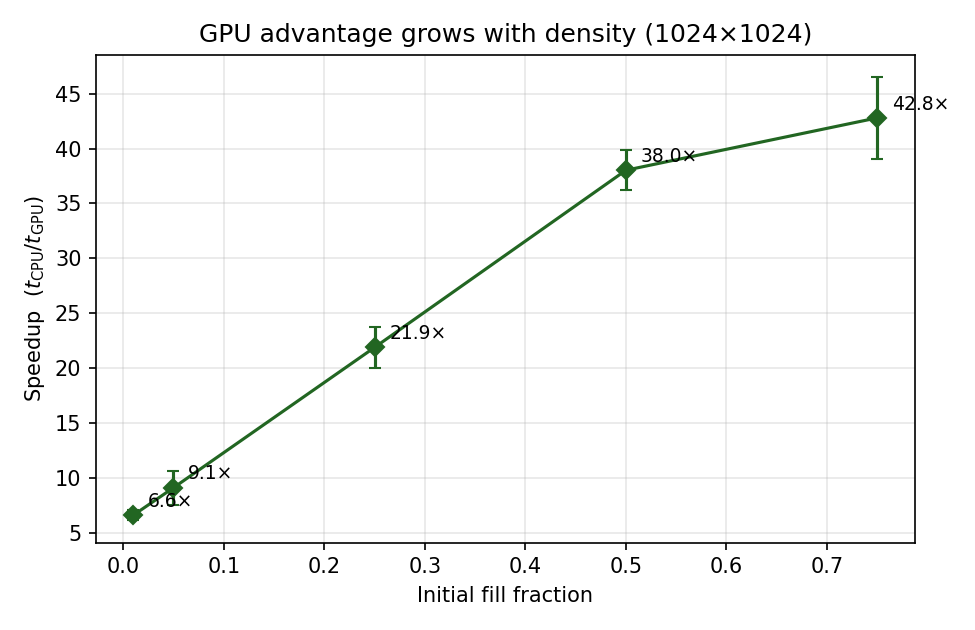
\includegraphics[width=0.6\linewidth]{figures/exp1b/exp1b_speedup.png}
  \label{fig:exp1b_speedup}
\end{center}

\paragraph{Interpretation.}
The speedup grows monotonically with density, from $6.6\times$ at
$1\%$ fill to $42.8\times$ at $75\%$, and the curve is visibly concave, so
the "gain per unit density" flattens toward the high-density end.
This demonstrates that no single ``speedup'' number characterises the
GPU implementation: the same hardware on the same grid produces different
advantage depending purely on
scene occupancy.

The trend follows from the cost models of the two implementations. The
CPU update short-circuits on any non-sand cell
(\texttt{if (read(r,c) != Sand) continue}), so its per-step cost is
approximately $a + b\rho$ in the active-grain density $\rho$, with $a$
a fixed overhead (snapshot copy, empty-cell scan) and $b$ the marginal
cost per grain. The GPU dispatches one invocation per $2\times 2$
block and executes the LUT update unconditionally, giving a
density-independent cost $c$ and a predicted speedup
$S(\rho)=(a+b\rho)/c$, linear in $\rho$ with positive intercept. The
observed sub-linearity at high density indicates that the CPU cost
itself ceases to be strictly linear in $\rho$ once the grid is densely
packed: many grains are blocked by their downward neighbours and exit
via the early-return paths in \texttt{simulation.cpp}, so the marginal
cost of an additional grain falls.


\section{Experiment 2 --- Conservation and directional symmetry}
\label{sec:exp2}


\paragraph{Setup}
A single filled disk of sand is seeded on the vertical midline
(centre column $W/2$, row $H/4$, radius $W/16$) and the
simulation is run until the pile has fully settled. The grid is then
partitioned into a strict left half (columns $0..W/2-1$) and strict
right half (columns $W/2+1..W-1$); the centre column $W/2$ is
\emph{excluded from both}, so the partition is invariant under
reflection about the midline. The seed is mirror-symmetric by
construction, giving $L_0=R_0$ exactly, which both implementations
assert before running. The bias metric is
\[
  \mathrm{rel\_diff} \;=\; \frac{L-R}{\text{total}},
\]
whose sign indicates the direction of any net horizontal drift.

\paragraph{Pass conditions} The CPU rule
is stochastic (a random tiebreak on symmetric diagonal choices) with an
additional deterministic symmetriser (column-scan direction alternates
each step). A single seed yields one trajectory, so even a perfectly
unbiased rule produces a residual $|\mathrm{rel\_diff}| \sim
1/\sqrt{N_{\text{grains}}}$ from sampling. It is
\begin{itemize}
    \item $\approx 3.5\%$ for the
$\approx 800$ grains at $W=256$
    \item $\approx 0.9\%$ for the
$\approx 12{,}800$ grains at $W=1024$
\end{itemize}
 A pass is a residual within this
noise floor. 

The GPU rule is fully deterministic, so its expected residual is exactly zero up to grains
landing in the excluded centre column; any sizeable constant would be a
genuine, reproducible bias in the tables.

\paragraph{Results}

\begin{table}[H]
  \centering
  \begin{tabular}{llrrrr}
    \toprule
    impl & $W$ & $L$ & $R$ & total & $\mathrm{rel\_diff}$ \\
    \midrule
    seq & 256  & 382  & 387  & 797   & $-0.00627$ \\
    gpu & 256  & 385  & 384  & 797   & $+0.00126$ \\
    seq & 1024 & 6373 & 6366 & 12853 & $+0.00055$ \\
    gpu & 1024 & 6364 & 6364 & 12853 & $\phantom{+}0.00000$ \\
    \bottomrule
  \end{tabular}
  \caption{Symmetry test results. \texttt{total} is identical across
    implementations at each size, confirming identical seeds and
    conservation.}
  \label{tab:exp2}
\end{table}

\begin{center}
  \begin{tabular}{ccc}
  
\includegraphics[width=0.4\linewidth]{figures/exp2b/cpu_256_rNA_exp2b.png} &
  
\includegraphics[width=0.4\linewidth]{figures/exp2b/gpu_256_r40_exp2b.png}
  \par\smallskip
  \label{fig:exp2b}
  \end{tabular}
  
  {\small \textit{Settled piles at $W=256$ for the CPU (left) and GPU (right)
    implementations. Both are symmetric about the midline.}}
\end{center}

All four configurations pass. The CPU residuals ($-0.63\%$ at $W=256$,
$+0.055\%$ at $W=1024$) sit comfortably inside the
$\sim 1/\sqrt{N_{\text{grains}}}$ noise floor and shrink with grid size,
as expected of sampling noise rather than systematic bias. The GPU
residual is a single grain at $W=256$ ($L-R=1$, with $28$ grains in the
excluded centre column) and exactly zero at $W=1024$
($L=R=6364$, $125$ grains in the centre column). The settled piles
 are symmetric pyramids peaked on the midline,
qualitatively confirming the quantitative result.


\newpage
\bibliographystyle{plain}
\bibliography{main}

\newpage
\appendix

\section{Appendix}
\label{sec:appendix}

\end{document}